\section{Software Architecture: Service Decomposition}

\subsection{Architectural Style}

The system follows a domain-oriented microservice style. The following rules
apply to every service and are not repeated in the work-stream sections:
\begin{itemize}
  \item \textbf{Database per service.} Only the owner writes its data; other
    services use its API or events, and cross-service references are logical
    IDs, never foreign keys.
  \item \textbf{Synchronous only when the caller needs the answer};
    everything else uses events delivered at least once through a
    transactional outbox to idempotent consumers.
  \item \textbf{No distributed transactions.} Cross-service workflows are
    sagas with idempotency keys and compensations.
  \item \textbf{Deny by default.} Every service validates the token locally
    and still authorizes the specific resource.
  \item \textbf{Audit before effect.} A sensitive administrative action is
    executed only after its audit record is confirmed; if the Audit Service is
    unavailable, the action fails closed.
\end{itemize}

% ------------------------- Payments and Refunds -------------------------
\begingroup
\setlength{\emergencystretch}{3em}
\subsubsection{Payments and Refunds}
\label{sec:pay-style}

This work stream handles every money movement: the payment of \emph{Book
Accommodation}, the refunds of \emph{Cancel Reservation} and \emph{Handle
Refunds}, and host payouts. The payment gateway is external: the platform only
orchestrates it and keeps the accounts. Card numbers never enter the system;
clients tokenize the card with the gateway and only the token is stored.

\paragraph{Requirements gap.} Delivery~1 (FR01--FR10) has no payment
requirement although three use cases depend on it. We propose \textbf{FR11}:
\emph{the system shall orchestrate the guest payment through the external
gateway and never charge a guest twice for the same reservation}; and
\textbf{FR12}: \emph{the system shall issue full or partial refunds and record
every charge, refund and payout in an auditable ledger that separates the
platform margin from the amount owed to the host}.

\begin{longtable}{@{}L{3.0cm}L{10.8cm}@{}}
\toprule
\textbf{Service} & \textbf{Responsibility} \\
\midrule
\endhead
\textbf{Payment Coordination} &
  Creates the payment of each reservation; asks the gateway to authorize,
  capture, void and refund; receives gateway webhooks. Does not compute prices,
  decide refund amounts or keep balances. \\
\addlinespace
\textbf{Ledger \& Payout} &
  Append-only double-entry ledger that splits each charge between host and
  platform margin, schedules and executes host payouts, and serves balances
  and reports. \\
\bottomrule
\caption{Services of Payments and Refunds.}
\label{tab:pay-services}
\end{longtable}

Gateway integration changes often while accounting rules must stay stable and
auditable; separating the ledger also means a slow ledger never blocks a
payment.

\paragraph{Payment states.} \texttt{AUTHORIZED} (money held), \texttt{PENDING}
(waiting for the bank or no answer yet), \texttt{DECLINED}, \texttt{FAILED}
(attempts exhausted or hold expired), \texttt{CAPTURED} (charged, point of no
return), \texttt{VOIDED} (hold released), \texttt{PARTIALLY\_\allowbreak
REFUNDED} and \texttt{REFUNDED}.

\paragraph{Booking flow.} It extends the reservation saga (10-minute hold in
\texttt{PENDING\_\allowbreak PAYMENT}):
\begin{enumerate}
  \item The Reservation Service calls \texttt{POST} \url{/api/v1/payments} with
    key \texttt{book:\allowbreak\{reservationId\}:\allowbreak auth:\allowbreak\{n\}}
    and the frozen \texttt{price\_\allowbreak snapshot}.
  \item Payment Coordination stores the payment and attempt \emph{before}
    calling the gateway, asks it to \textbf{hold} the money (at most
    $\approx$0.8\,s) and answers \texttt{201 AUTHORIZED}, \texttt{402 DECLINED}
    or \texttt{202 PENDING}, publishing \texttt{PaymentSucceeded} or
    \texttt{PaymentFailed}.
  \item On \texttt{Reservation\allowbreak Confirmed} it \textbf{captures} the money and
    publishes \texttt{PaymentCaptured}; the Ledger writes one balanced journal
    transaction.
  \item About 24\,h after check-in, as Airbnb does~\cite{airbnb-payouts}, the
    Ledger pays the host.
\end{enumerate}
A \textbf{declined} payment is not retried automatically: the guest may try
another method while the hold lasts, and after three declines the payment is
\texttt{FAILED}. A \textbf{pending} payment is resolved by webhook or by a
reconciler that runs every 5 minutes; a timeout is never treated as a failure
because the money may have moved. On \texttt{Reservation\allowbreak Expired} any
authorization is voided.

\paragraph{Refunds.} On cancellation the Reservation Service applies its
policy and calls \texttt{POST} \url{/api/v1/refunds}; an uncaptured payment is
voided instead. A gateway rejection does not undo the cancellation; it opens a
support case. Manual refunds are requested by a support agent, who chooses who
funds them, and are audited before effect.

\begin{figure}[H]
  \centering
  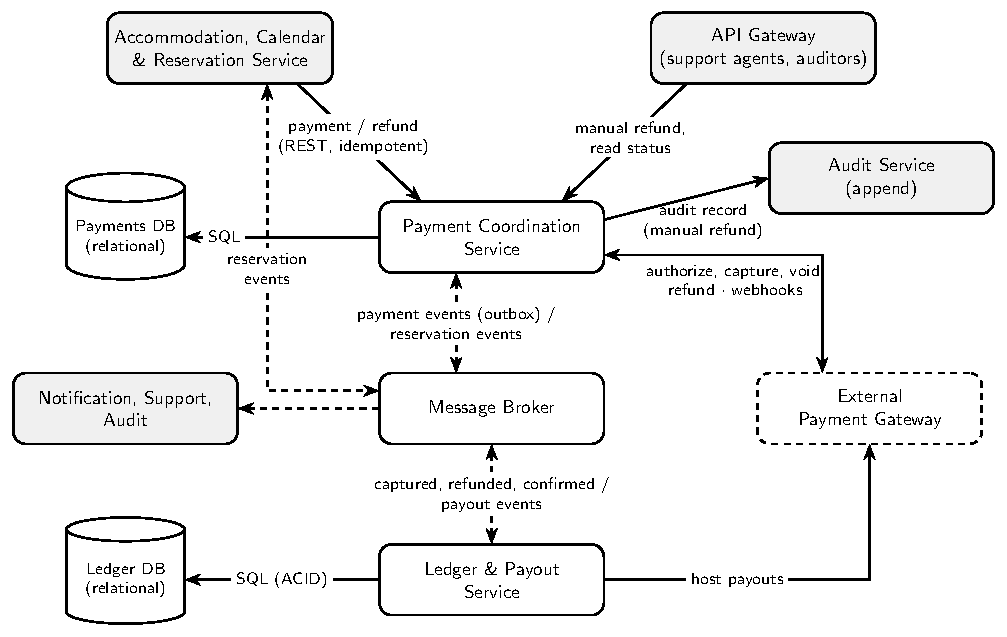
\includegraphics[width=\linewidth]{images/payments_components.pdf}
  \caption{Payments and Refunds components.}
  \label{fig:pay-components}
\end{figure}
\endgroup

% ------------------------- Reservation and Calendar -------------------------
\subsubsection{Reservation and Calendar}
\label{sec:res-style}

The \textbf{Reservation and Accommodation Service} owns accommodations, the
availability calendar (holds, reservations and host blocks), reservations and
check-in/out agreements. It covers \emph{Book Accommodation}, \emph{Cancel
Reservation}, \emph{Manage Reservations}, \emph{Manage Accommodation Listing}
and the administrative pause of listings (FR01--FR06, FR10). Holds and listing
saves are synchronous; booking and payment form a saga. When a host creates or
edits a listing, the service requests the pricing multiplier and stores it.

\begin{figure}[H]
\centering
\begin{tikzpicture}[
  scale=0.72, transform shape,
  font=\sffamily\small,
  >={Stealth[length=2.5mm]},
  svc/.style={draw, thick, rounded corners=6pt, minimum width=3.6cm,
              minimum height=1.2cm, align=center, fill=white},
  oth/.style={svc, fill=gray!12},
  ext/.style={svc, dashed},
  db/.style={cylinder, shape border rotate=90, draw, thick, aspect=0.25,
             minimum width=1.9cm, minimum height=1.8cm, align=center, fill=white,
             font=\sffamily\footnotesize},
  flow/.style={->, dashed, thick},
  sync/.style={->, thick},
  lbl/.style={fill=white, inner sep=2pt, align=center, font=\sffamily\footnotesize}
]
  \node[oth] (apigw) at (0, 5.5)  {API Gateway};
  \node[svc] (res)   at (0, 1.5)  {Reservation and\\Accommodation Service\\(listings, calendar,\\reservations)};
  \node[db]  (resdb) at (0,-2.8)  {Service DB\\(PostgreSQL)};
  \node[oth] (price) at (-6, 1.5) {Pricing\\Service};
  \node[oth] (pay)   at (6, 1.5)  {Payment\\Coordination};
  \node[ext] (gate)  at (6,-2.8)  {External\\Payment Gateway};
  \node[svc] (broker) at (6, 5.5) {Message Broker};
  \node[oth] (cons)  at (-6, 5.5) {Search, Notification,\\Support and Admin.};
  \node[svc] (timer) at (-6,-2.8) {Hold timer\\(scheduler, sweeper)};

  \draw[sync] (apigw.south) -- node[lbl]{REST} (res.north);
  \draw[sync] (res.south) -- node[lbl]{SQL\\(ACID)} (resdb.north);
  \draw[sync, <->] (res.west) -- node[lbl]{multiplier request /\\occupancy query} (price.east);
  \draw[sync] (res.east) -- node[lbl]{payment\\intent} (pay.west);
  \draw[sync, <->] (pay.south) -- node[lbl]{charge /\\refund} (gate.north);
  \draw[flow, <->] (broker.south west) -- node[lbl, pos=0.45]{reservation and\\payment events} (res.north east);
  \draw[flow] (pay.north) -- node[lbl, pos=0.55]{payment\\events} (broker.south);
  \draw[flow] (broker.north) -- ++(0,0.9) -| (cons.north);
  \node[lbl] at (0,6.4) {listing, reservation and availability events};
  \draw[flow] (timer.north) -- node[lbl, pos=0.4]{HoldExpired} (res.south west);
  \draw[flow] (timer.east) -- node[lbl, above=2pt]{expired holds} (resdb.west);
\end{tikzpicture}
\caption{Reservation and Accommodation Service.}
\end{figure}

% ------------------------- Pricing Engine -------------------------
\begingroup
\setlength{\emergencystretch}{3em}
\subsubsection{Pricing Engine}
\label{sec:price-style}

This work stream computes the \textbf{pricing multiplier} of each
accommodation (FR03): 1.02, 1.07 or 1.15. Applied to the host's base price it
gives the effective nightly rate, and it is also the platform margin used by
Payments (Section~\ref{sec:pay-model}). It is requested synchronously when a
listing is created or edited and then frozen in each reservation, so the
engine never changes the price of an existing booking.

\paragraph{Computation.} Each request is answered from a \textbf{precomputed
zone snapshot}, without calling other services:
\begin{itemize}
  \item \textbf{Demand} (daily, per zone): occupancy of the next 90 days,
    booking pace (last 7 days) and a search index (searches of the last 7 days
    against the 4-week average).
  \item \textbf{Context} (monthly, per zone): impact score (0--1) of local
    events obtained from SerpAPI.
  \item \textbf{Listing} (from the request): maximum guests, base price and
    whether cleaning is included.
\end{itemize}
The score $0.6\cdot$demand $+\ 0.3\cdot$context $+\ 0.1\cdot$listing maps to
\texttt{LOW} (1.02), \texttt{STANDARD} (1.07) or \texttt{HIGH} (1.15). Weights
and thresholds form a \textbf{model version} that becomes active only after an
administrator approves it. A zone without snapshot gets \texttt{STANDARD} with
\texttt{fallback = true}, so a listing save never fails for lack of data.

\begin{longtable}{@{}L{3.2cm}L{10.6cm}@{}}
\toprule
\textbf{Service} & \textbf{Responsibility} \\
\midrule
\endhead
\textbf{Pricing Service} &
  \texttt{pricing-api} answers the multiplier, records each calculation and
  manages model versions; \texttt{pricing-worker} applies indicator events to
  the snapshot and archives old history. \\
\addlinespace
\textbf{Demand Indicators} &
  Counts search events per zone and, daily, reads calendar occupancy;
  publishes \texttt{Demand\allowbreak Indicators\allowbreak Updated}. \\
\addlinespace
\textbf{Context Indicators} &
  Monthly SerpAPI job that publishes \texttt{Context\allowbreak Indicators\allowbreak Updated};
  isolates the only external dependency. \\
\bottomrule
\caption{Services of the Pricing Engine.}
\label{tab:price-services}
\end{longtable}

Indicator ingestion is separated from the request path so that search traffic
and the external API never affect the latency of a listing save.

\begin{figure}[H]
  \centering
  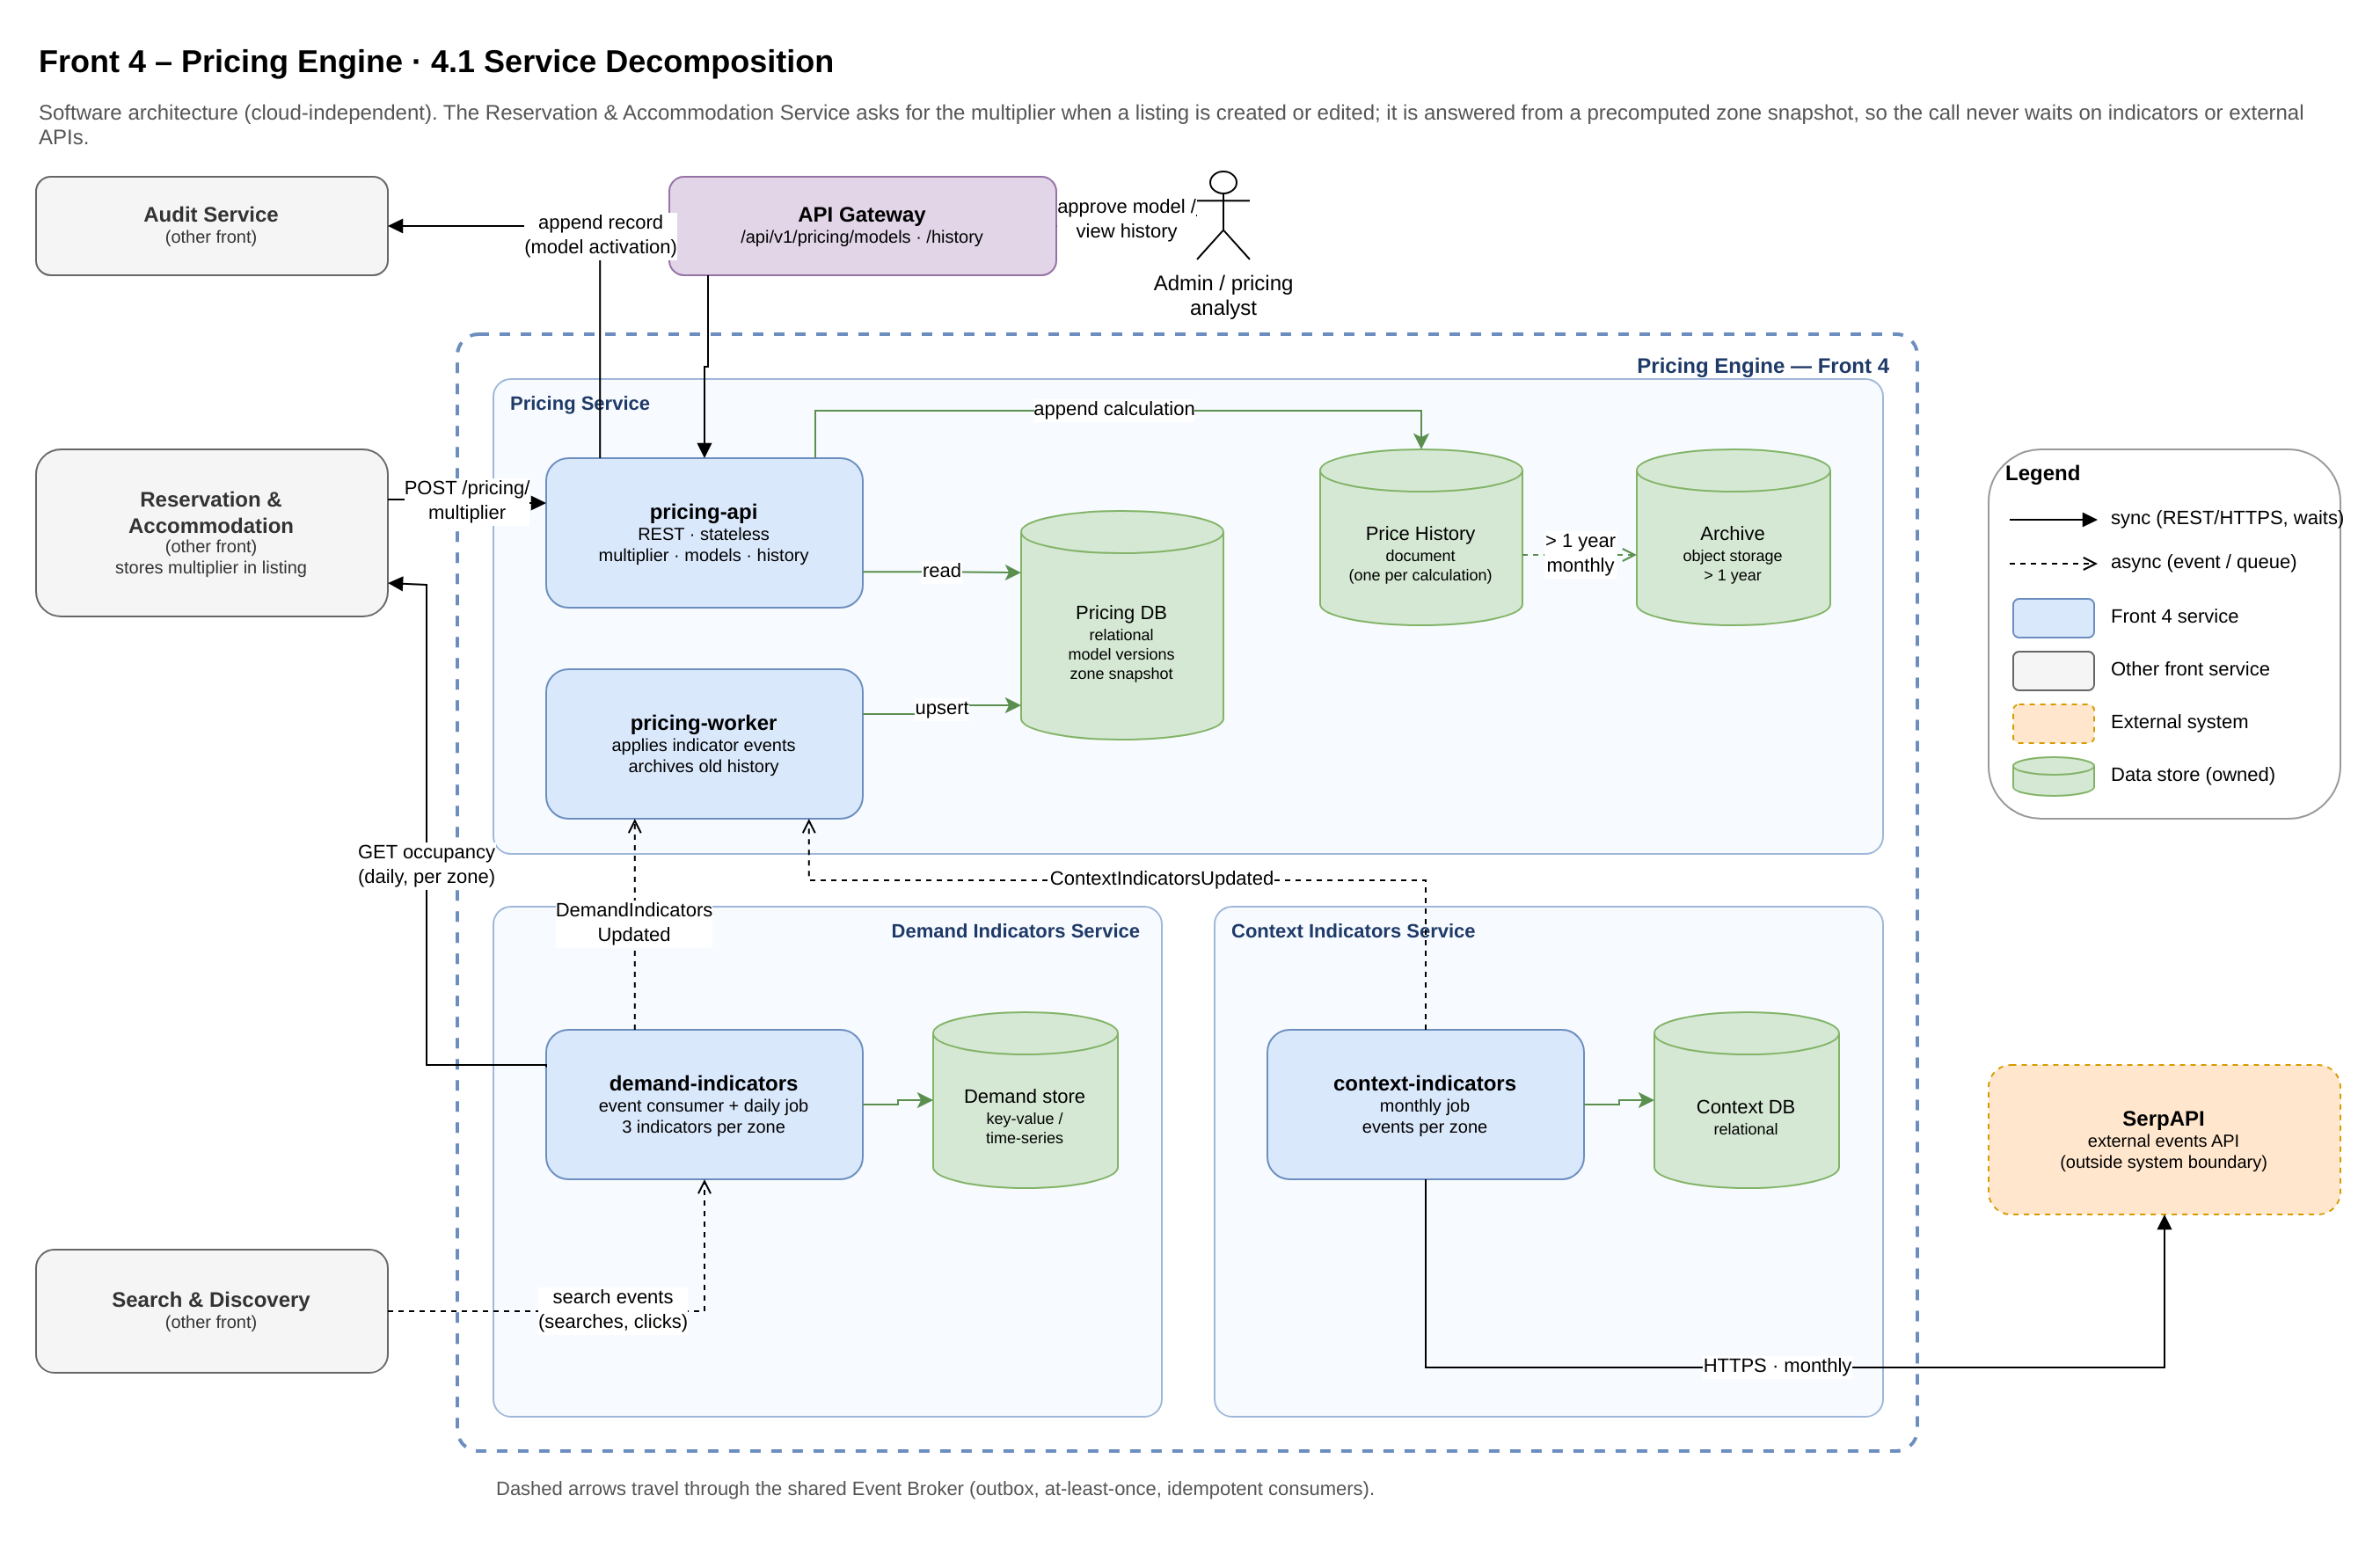
\includegraphics[width=\linewidth]{images/pricing_41_service_decomposition.png}
  \caption{Pricing Engine components.}
  \label{fig:price-components}
\end{figure}
\endgroup

% ------------------------- Identity, Communication and Internal Operations -------------------------
\begingroup
\setlength{\emergencystretch}{3em}
\subsubsection{Identity, Communication and Internal Operations}
\label{sec:id-style}

This work stream covers authentication and role-based access (FR09, FR10),
guest--host messaging, notifications, support cases, privileged administration
and the immutable audit trail. Visitors reach only public pages, registration
and login; guests and hosts reach only their own resources; administrators,
auditors and support agents require MFA, and administrators also need a fresh
step-up for sensitive actions.

\begin{longtable}{@{}L{3.1cm}L{10.7cm}@{}}
\toprule
\textbf{Service} & \textbf{Responsibility} \\
\midrule
\endhead
\textbf{Identity \& Access} &
  Registration, login, tokens, MFA, password reset, session revocation and
  public signing keys. \\
\textbf{User Profile} &
  Profile, contact data, role and account status (no credentials). \\
\textbf{Messaging} &
  Conversations, history, read state and real-time delivery. \\
\textbf{Notification} &
  Channels, templates, preferences, retries, fallback and duplicate
  suppression. \\
\textbf{Support} &
  Support cases, assignment and transitions; never executes refunds. \\
\textbf{Administration} &
  Privileged workflows (Manage Users, Manage Accommodations); owns no business
  data and delegates each change to its owner. \\
\textbf{Audit} &
  Append-only, hash-chained records and read-only queries. \\
\bottomrule
\caption{Services of Identity, Communication and Internal Operations.}
\label{tab:id-services}
\end{longtable}

Credentials and profiles have different security and scaling needs; a message
must be stored even if every notification channel is down; casework is not
privileged administration; and audit evidence needs its own retention and
read-only access. These reasons define the seven boundaries.

\begin{figure}[H]
  \centering
  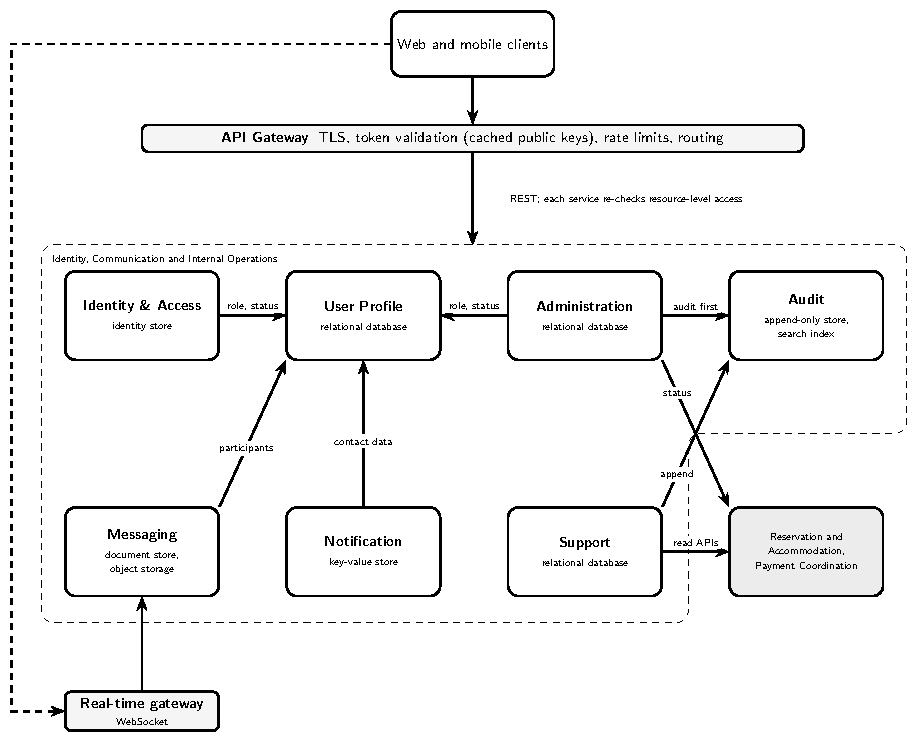
\includegraphics[width=\linewidth]{images/identity_components.pdf}
  \caption{Identity, Communication and Internal Operations components
  (events are shown in Figure~\ref{fig:id-events}).}
  \label{fig:id-components}
\end{figure}
\endgroup

\paragraph{Diagram conventions.} In all component diagrams, solid arrows are
synchronous calls, dashed arrows are events, grey boxes belong to other work
streams and dashed boxes are external systems.

% =====================================================================
\subsection{API Contracts}

Public paths are versioned under \texttt{/api/v1} and internal paths under
\texttt{/internal/v1}; internal endpoints accept only service identities.
Every money-moving request carries an \texttt{Idempotency-Key} header. The
standard codes \texttt{400}, \texttt{403} and \texttt{404} apply to every
endpoint and are listed only when they carry a specific meaning.

% ------------------------- Payments and Refunds -------------------------
\begingroup
\setlength{\emergencystretch}{3em}
\subsubsection{Payments and Refunds}
\label{sec:pay-api}

\begin{longtable}{@{}L{1.5cm}L{4.8cm}L{2.3cm}L{5.0cm}@{}}
\toprule
\textbf{Method} & \textbf{Endpoint} & \textbf{Caller} & \textbf{Purpose and codes} \\
\midrule
\endhead
\multicolumn{4}{@{}l}{\emph{Payment Coordination}} \\
POST & \url{/api/v1/payments} & Reservation &
  Create the payment and hold the money. \texttt{201} authorized,
  \texttt{202} pending, \texttt{402} declined, \texttt{409} same key in
  progress, \texttt{422} same key, other body. \\
POST & \url{/api/v1/payments/{id}/attempts} & Guest &
  Retry with another method; \texttt{409} attempts exhausted. \\
GET & \url{/api/v1/payments/{id}} & Guest, Support & Payment state. \\
POST & \url{/api/v1/refunds} & Reservation, support agent &
  Cancellation refund, or manual refund with case, reason and
  \texttt{fundedBy}. \texttt{202}; \texttt{400} above refundable balance. \\
GET & \url{/api/v1/refunds/{id}} & Guest, support agent & Refund state. \\
POST & \url{/api/v1/payments/webhooks/gateway} & Gateway &
  Signed notification. \texttt{200} (also duplicates), \texttt{401} bad
  signature. \\
\addlinespace
\multicolumn{4}{@{}l}{\emph{Ledger \& Payout}} \\
GET & \url{/api/v1/ledger/hosts/{id}/balance}, \url{.../payouts} & Host, admin &
  Earnings and payout history. \\
GET & \url{/api/v1/ledger/reservations/{id}/entries} & Support, auditor &
  Accounting entries of a reservation. \\
GET & \url{/api/v1/ledger/reconciliation?date=} & Auditor, admin &
  Ledger vs.\ gateway settlement. \\
\bottomrule
\caption{API of Payments and Refunds.}
\label{tab:pay-api}
\end{longtable}
\endgroup

% ------------------------- Reservation and Calendar -------------------------
\subsubsection{Reservation and Calendar}
\label{sec:res-api}

\begin{table}[!ht]
  \centering
  \footnotesize
  \begin{tabularx}{\textwidth}{@{}>{\raggedright\arraybackslash}p{5.6cm}>{\raggedright\arraybackslash}p{2.0cm}>{\raggedright\arraybackslash}X>{\raggedright\arraybackslash}p{1.6cm}@{}}
    \toprule
    \textbf{Method and path} & \textbf{Access} & \textbf{Purpose} & \textbf{Codes} \\
    \midrule
    \texttt{POST /listings} & Host & Create; calls Pricing and stores the multiplier & 201, 502 \\
    \texttt{PATCH /listings/\{id\}} & Owner & Edit (with \texttt{version}); re-prices if needed & 200, 409, 502 \\
    \texttt{GET /listings/\{id\}} & Public & Details and effective rate & 200 \\
    \texttt{POST|DELETE /listings/\{id\}/calendar/blocks} & Owner & Block or release dates (FR02) & 201/200, 409 \\
    \texttt{GET /admin/listings} & Admin, Support & Search by zone, status, host & 200 \\
    \texttt{PATCH /admin/listings/\{id\}/status} & Admin & Pause or reactivate & 200, 409 \\
    \texttt{POST /reservations} & Guest & Hold and payment intent & 201, 409, 422 \\
    \texttt{GET /reservations[/\{id\}]} & Parties, Support & Reservation details or host's list & 200 \\
    \texttt{POST /reservations/\{id\}/cancel} & Guest, host, admin & Cancel and request refund & 200, 409 \\
    \texttt{PATCH /reservations/\{id\}/agreements} & Guest, host & Check-in/out agreement (FR05) & 200, 409 \\
    \texttt{GET /internal/v1/calendar/occupancy} & Internal & Booked and blocked nights per zone & 200 \\
    \bottomrule
  \end{tabularx}
  \caption{API of the Reservation and Accommodation Service.}
\end{table}

% ------------------------- Pricing Engine -------------------------
\begingroup
\setlength{\emergencystretch}{3em}
\subsubsection{Pricing Engine}
\label{sec:price-api}

\begin{longtable}{@{}L{1.5cm}L{4.8cm}L{2.3cm}L{5.0cm}@{}}
\toprule
\textbf{Method} & \textbf{Endpoint} & \textbf{Caller} & \textbf{Purpose and codes} \\
\midrule
\endhead
POST & \url{/api/v1/pricing/multiplier} & Reservation &
  Returns \texttt{multiplier}, \texttt{tier}, \texttt{effective\allowbreak Nightly\allowbreak Rate},
  \texttt{modelVersion}, \texttt{fallback}. Read-only and deterministic, so
  retries are safe. \texttt{200}. \\
GET & \url{/api/v1/pricing/listings/{id}/history} & Owner host, admin &
  Past calculations with the indicators used. \\
GET, POST & \url{/api/v1/pricing/models} & Analyst, admin &
  List versions; propose one in \texttt{DRAFT}. \\
POST & \url{/api/v1/pricing/models/{v}/approve} & Admin (step-up) &
  Approve and activate. \texttt{409} not \texttt{DRAFT}, \texttt{503} audit
  unavailable. \\
GET & \url{/internal/v1/demand-indicators?zoneId=}, \url{/internal/v1/context-indicators?zoneId=} &
  Pricing & Latest indicators of a zone (snapshot rebuild). \\
\bottomrule
\caption{API of the Pricing Engine.}
\label{tab:price-api}
\end{longtable}

{\footnotesize
\begin{verbatim}
POST /api/v1/pricing/multiplier
{ "listingId": "lst-5521", "zoneId": "bog-chapinero", "maxGuests": 4,
  "basePrice": 250000, "includesCleaning": true }
200 { "multiplier": 1.07, "tier": "STANDARD", "effectiveNightlyRate": 267500,
      "modelVersion": "v3", "fallback": false }
\end{verbatim}
}
\endgroup

% ------------------------- Identity, Communication and Internal Operations -------------------------
\begingroup
\setlength{\emergencystretch}{3em}
\subsubsection{Identity, Communication and Internal Operations}
\label{sec:id-api}

Only the main endpoints are listed; the rest (logout, password reset, devices,
comments, integrity proofs) follow the same rules.

\begin{longtable}{@{}L{1.5cm}L{4.8cm}L{2.5cm}L{4.8cm}@{}}
\toprule
\textbf{Method} & \textbf{Endpoint} & \textbf{Caller} & \textbf{Purpose and codes} \\
\midrule
\endhead
POST & \url{/api/v1/auth/register} & Visitor &
  Create credential, start profile saga. \texttt{201}, \texttt{409}. \\
POST & \url{/api/v1/auth/login} & Visitor &
  Issue tokens. \texttt{200}, \texttt{401}, \texttt{429}. \\
POST & \url{/api/v1/auth/mfa/verify} & Privileged &
  Second factor or step-up. \texttt{200}, \texttt{401}. \\
GET & \url{/api/v1/auth/jwks} & Gateway, services & Public signing keys. \\
GET & \url{/internal/v1/users/{id}/authorization} & Identity \& Access &
  Role and status at login. \\
PATCH & \url{/internal/v1/users/{id}/role} & Administration &
  Change role. \texttt{409}. \\
POST, GET & \url{/api/v1/conversations/{id}/messages} & Participant &
  Send (stored before answering) or read history. \\
WS & \url{/realtime} & Guest, host & Real-time delivery. \\
PUT & \url{/api/v1/notification-preferences} & User & Consent per channel. \\
POST & \url{/internal/v1/notifications} & Services & Enqueue. \texttt{202}. \\
POST, GET, PATCH & \url{/api/v1/support/cases[/{id}]} & Reporter, Support &
  Open, read or update a case. \texttt{409} stale version, \texttt{422}
  invalid transition. \\
PATCH & \url{/api/v1/admin/users/{id}/role}, \url{/api/v1/admin/accommodations/{id}/status} &
  Admin (step-up) & Change a role or pause a listing with a reason.
  \texttt{202}, \texttt{503} audit unavailable. \\
POST & \url{/internal/v1/audit/records} & Sensitive services &
  Append (idempotent). \texttt{201}, \texttt{503}. \\
GET & \url{/api/v1/audit/records} & Auditor & Query records. \\
\bottomrule
\caption{Main API of Identity, Communication and Internal Operations.}
\label{tab:id-api}
\end{longtable}
\endgroup

% =====================================================================
\subsection{Data Owned}

Each service is the only writer of its data (Table~\ref{tab:data-owned}).
Data used by several work streams is never duplicated as an authority: prices
are frozen in the reservation, availability is decided only by the calendar,
and business events belong to their producers.

\begin{longtable}{@{}L{3.6cm}L{10.2cm}@{}}
\toprule
\textbf{Service} & \textbf{Data owned} \\
\midrule
\endhead
\multicolumn{2}{@{}l}{\emph{Payments and Refunds}} \\
Payment Coordination & Payments, attempts, refunds, idempotency records,
  gateway inbox, outbox; only the card token. \\
Ledger \& Payout & Accounts, journal transactions and entries
  (append-only), payouts. \\
\addlinespace
\multicolumn{2}{@{}l}{\emph{Reservation and Calendar}} \\
Reservation and Accommodation & Accommodations (with multiplier and
  effective rate), calendar entries, reservations with price and condition
  snapshots, status history, check-in/out agreements, outbox. \\
\addlinespace
\multicolumn{2}{@{}l}{\emph{Pricing Engine}} \\
Pricing & Model versions, zone snapshot, calculation history and archive. \\
Demand Indicators & Search counters and demand snapshots per zone. \\
Context Indicators & Fetch runs and context events. \\
\addlinespace
\multicolumn{2}{@{}l}{\emph{Identity, Communication and Internal Operations}} \\
Identity \& Access & Hashed credentials, MFA factors, sessions, signing keys,
  revocations. \\
User Profile & Profiles, contact data, roles, account status. \\
Messaging & Conversations, messages, read state, attachments (object
  storage). \\
Notification & Preferences, devices, templates, delivery attempts. \\
Support & Cases, comments, transitions. \\
Administration & Administrative actions, approvals, policies. \\
Audit & Audit records, integrity anchors, search index. \\
\bottomrule
\caption{Data owned by each service.}
\label{tab:data-owned}
\end{longtable}

% =====================================================================
\subsection{Dependencies}

Table~\ref{tab:dependencies} lists the dependencies between work streams.
Every service also depends on Identity \& Access for token validation (local,
with cached public keys) and on the broker for events; these are omitted.

\begin{longtable}{@{}L{3.2cm}L{3.6cm}L{7.0cm}@{}}
\toprule
\textbf{Service} & \textbf{Depends on} & \textbf{Why} \\
\midrule
\endhead
Reservation & Pricing (sync) &
  Multiplier on listing create or edit; failure returns \texttt{502} to the
  host. \\
Reservation & Payment Coordination (sync + events) &
  Payment intent and refunds; confirms on \texttt{PaymentSucceeded}. \\
Payment Coordination, Ledger & Reservation (events) &
  Capture, void, refund and payout scheduling follow reservation events. \\
Payment Coordination, Ledger & Pricing (indirect) &
  The frozen multiplier is the platform margin; no direct call. \\
Payment Coordination, Ledger & External gateway &
  Authorize, capture, void, refund, payout; webhooks. \\
Demand Indicators & Reservation (sync), Search (events) &
  Daily calendar occupancy; search events per zone. \\
Context Indicators & SerpAPI &
  Monthly local events; on failure the last data is kept. \\
Payments, Pricing, Admin., Identity, Support & Audit (sync) &
  Sensitive actions fail closed without a confirmed record. \\
Pricing (approval), Administration & Identity \& Access &
  Step-up MFA for sensitive actions. \\
Administration & Reservation, User Profile &
  Delegates listing pauses and role changes to their owners. \\
Support & Reservation, Payment Coordination &
  Reads case context and refund status; consumes
  \texttt{Refund\allowbreak Status\allowbreak Changed}. \\
Notification, Search, Audit & All producers (events) &
  User messages, search index refresh, audit trail. \\
Notification & Email, push, SMS providers & Channel delivery. \\
\bottomrule
\caption{Dependencies between work streams.}
\label{tab:dependencies}
\end{longtable}

% =====================================================================
\subsection{Scaling Characteristics}

All application services are stateless and scale horizontally; workers scale
on queue depth. Table~\ref{tab:scaling} gives the estimated instances at real
scale (Delivery~1 load: booking and payment 5\,\%, about 13 req/s average and
130 at peak; authentication 8\,\%, 21/208 req/s; messaging 4\,\%, 10/104
msg/s; search 60\,\%). In the academic simulation one instance per service
plus one replica for availability is enough.

\begin{longtable}{@{}L{3.4cm}L{6.6cm}L{1.8cm}L{1.8cm}@{}}
\toprule
\textbf{Service} & \textbf{Scaling driver and notes} & \textbf{Average} & \textbf{Peak} \\
\midrule
\endhead
Payment Coordination & I/O-bound: $\approx$1\,s per gateway call, about 130
  requests in flight at peak, $\approx$40 per instance, plus one spare & 2 & 6 \\
Ledger \& Payout & Queue depth; off the guest's path & 2 & 2 \\
Reservation & Request rate and p95; the limit is contention on a single
  listing, enforced by the database, not volume. Calendar reads can use a
  replica & 1 & 2 \\
\texttt{pricing-api} & Only on listing writes; one indexed read plus one
  append, p95 target 150\,ms & 1 & 2 \\
\texttt{pricing-worker} & Queue depth & 1 & 1 \\
Demand Indicators & Queue depth of search events (counter increments) & 1 & 2 \\
Context Indicators & Monthly batch, only while running & 1 & 1 \\
Identity \& Access & CPU (slow password hashing at login) & 4 & 20 \\
User Profile & Read-heavy, cached by callers & 4 & 16 \\
Messaging & Requests and open connections (stateful real-time tier) & 4 & 20 \\
Notification & Queue depth and provider rate limits; one event fans out
  to several channels & 4 & 40 \\
Support & Low request volume & 2 & 6 \\
Administration & Very low volume; availability only & 2 & 4 \\
Audit & Append rate; index updated asynchronously & 2 & 8 \\
\bottomrule
\caption{Estimated instances per service at real scale.}
\label{tab:scaling}
\end{longtable}
